% !TeX root = ../../tesis.tex

% =============================================================================
%  4.2 — VISIÓN GENERAL
% =============================================================================
\section{VFTModel: El Motor Analítico de la Red}
\label{sec:vftmodel-intro}

\textbf{VFTModel} (\termino{Vanishing Fig-Tree Model}) es el segundo componente
de la arquitectura de código de esta investigación. Si \textbf{Apimetro} cumple
la función de fuente de datos —exponiendo la geometría de la red de transporte
mediante una \api{} \textsc{rest}—, VFTModel es el \textbf{motor analítico} que
consume esos datos, los transforma en una estructura matemática de grafos y
ejecuta los algoritmos que producen los indicadores topológicos presentados en
el Capítulo~\ref{ch:analisis-red-actual}.

\begin{figure}[htbp]
  \centering
  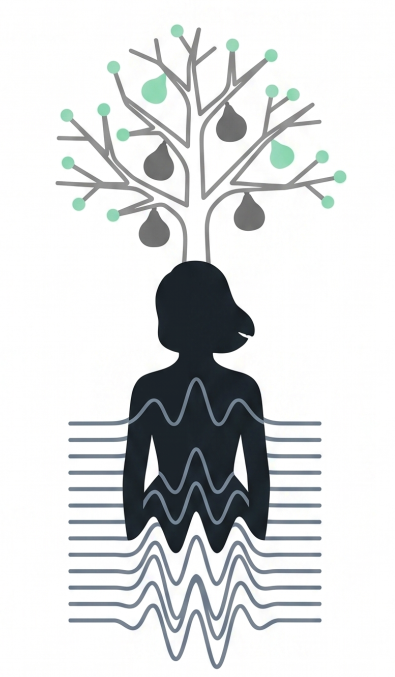
\includegraphics[width=0.2\textwidth]{Figures/Cap4/VFTLogo1.png}
  \caption[Ícono Personal de VFTModel]{Ícono Creado para el proyecto VFTModel}
  \label{fig:VFTModel-icon}
  \fuentefigura{Elaboración propia.}
\end{figure}


\subsection{Contexto y Motivación}
\label{subsec:vft-contexto}

La \zmvm{} alberga una de las redes de transporte público más heterogéneas del
mundo: desde el Metro, que opera en vías exclusivas subterráneas a velocidades
comerciales de hasta 36~km/h, hasta los Corredores Concesionados que comparten
carril con el automóvil particular y absorben la saturación vial de la ciudad.
Esta diversidad opera simultáneamente como fortaleza y como desafío analítico.
Contabilizar kilómetros de línea o número de estaciones no es suficiente para
determinar si la red es eficiente: un sistema puede tener muchas estaciones y
aun así obligar a sus usuarios a recorrer trayectos tortuosos, o concentrar toda
la conectividad en grandes nodos de transbordo mientras las zonas periféricas
quedan sin alimentación capilar adecuada.

VFTModel nace como respuesta a esta necesidad: un motor analítico de código
abierto y matemáticamente fundamentado, capaz de cuantificar la eficiencia
estructural de la red mediante indicadores topológicos derivados de la teoría de
grafos \citep{newman2010networks}. Su diseño prioriza la reproducibilidad:
cualquier investigador con acceso a datos \gtfs{} de una red urbana puede
replicar el análisis siguiendo la guía del Anexo~\ref{anx:vft-replicabilidad}.
El modelo transforma los datos geográficos del sistema metropolitano en una
estructura matemática de nodos y aristas sobre la cual aplica algoritmos de
análisis de redes, produciendo métricas concretas y comparables que permiten
evaluar la conectividad del sistema e identificar nodos vulnerables.

\subsection{El Nombre: Vanishing Fig-Tree}
\label{subsec:vft-nombre}

La denominación \termino{Vanishing Fig-Tree} —árbol de higuera en desaparición o
Modelo de la Higuera Evanescente— es una metáfora del comportamiento topológico
de una red de transporte fragmentada.
\\
\termino{Vanishing Fig-Tree Model} se basa en dos referencias clave en
diferentes ámbitos: una es literaria y describe la desesperanza de una situación
crítica ante una decisión tan trascendente, mientras que la otra describe de
manera lírica el llamado \termino{Punto de No Retorno}:

\citaclave{
  \begin{center}
``From the tip of every branch, like a fat purple fig, a wonderful future
beckoned and
winked. One fig was a husband and a happy home and children, and another fig was
a famous
poet and another fig was a brilliant professor, and another fig was Europe and
Africa and
South America, and another fig was Constantine and Socrates and Attila and a
pack of other
lovers with queer names and offbeat professions, and another fig was an Olympic
lady crew
champion, and beyond and above these figs were many more figs I couldn't quite
make out.
    \\ \vspace{1ex}
I saw myself sitting in the crotch of this fig tree, starving to death, just
because
I couldn't make up my mind which of the figs I would choose. I wanted each and
every
one of them, but choosing one meant losing all the rest, and, as I sat there,
unable
to decide, the figs began to wrinkle and go black, and, one by one, they plopped
    to the ground at my feet.''

    \vspace{1.5ex}
    \hrule
    \vspace{1.5ex}

``De la punta de cada rama, como si de un grueso higo morado se tratara, pendía
un
maravilloso futuro, señalado y rutilante. Un higo era un marido y un hogar feliz
e
hijos y otro higo era un famoso poeta, y otro higo era un brillante profesor, y
otro
higo era Europa y África y Sudamérica y otro higo era Constantino y Sócrates y
Atila
y un montón de otros amantes con nombres raros y profesionales poco usuales, y
otro
higo era una campeona de equipo olímpico de atletismo, y más allá y por encima
de
    aquellos higos había muchos más higos que no podía identificar claramente.
    \\ \vspace{1ex}
Me vi a mí misma sentada en la bifurcación de ese árbol de higos, muriéndome de
hambre sólo porque no podía decidir cuál de los higos escoger. Quería todos y
cada
uno de ellos, pero elegir uno significaba perder el resto, y, mientras yo estaba
allí
sentada, incapaz de decidirme, los higos empezaron a arrugarse y a tornarse
negros y,
    uno por uno, cayeron al suelo, a mis pies.'' \\
    \vspace{1ex}
    \citep{plath2019campana}
  \end{center}
}

\citaclave{
  \begin{center}
    ``My life ain't no holiday \\
    I've been through the point of no return \\
    I've seen what a man can do \\
    I've seen all the hate of a woman too.''

    \vspace{1.5ex}
    \hrule
    \vspace{1.5ex}

    ``Mi vida no es ninguna vacación \\
    He cruzado el punto de no retorno \\
    He visto lo que un hombre puede hacer \\
    También he visto todo el odio de una mujer.'' \\
    \vspace{1ex}
    \citep{neworder_vanishingpoint_1989}
  \end{center}
}

Una higuera no muere cuando pierde sus ramas más delgadas. El tronco y las ramas
principales permanecen, pero su capacidad de expansión y de alimentación colapsa
silenciosamente: las raíces capilares dejan de nutrir las zonas más alejadas, y
el árbol entra en una decadencia progresiva que no es visible desde el exterior
hasta que es demasiado tarde. De manera análoga, una red de transporte puede
mantener sus corredores troncales operativos con plena visibilidad pública,
mientras sus rutas de alimentación capilar desaparecen o se deterioran sin que
ese deterioro aparezca en los indicadores convencionales de pasajeros
transportados o kilómetros de línea. Las zonas que pierden su conexión capilar
quedan aisladas funcionalmente del resto del sistema, aunque sigan figurando en
los mapas oficiales.

El modelo propone medir precisamente esta fragilidad estructural mediante
indicadores que capturen tanto la conectividad interna de los nodos —la
\termino{Fuerza Capilar}— como la eficiencia de los recorridos reales frente a
la distancia teórica mínima —el \termino{Factor de Desviación}—, y el impacto
que tendría la pérdida de un nodo crítico sobre el sistema en su conjunto.
